\documentclass[journal,12pt,twocolumn]{IEEEtran}

\usepackage{setspace}
\usepackage{gensymb}
\singlespacing
\usepackage[cmex10]{amsmath}
\usepackage{amsthm}

\usepackage{mathrsfs}
\usepackage{txfonts}
\usepackage{stfloats}
\usepackage{bm}
\usepackage{cite}
\usepackage{cases}
\usepackage{subfig}

\usepackage{longtable}
\usepackage{multirow}

\usepackage{enumitem}
\usepackage{mathtools}
\usepackage{steinmetz}
\usepackage{tikz}
\usepackage{circuitikz}
\usepackage{verbatim}
\usepackage{tfrupee}
\usepackage[breaklinks=true]{hyperref}
\usepackage{graphicx}
\usepackage{tkz-euclide}

\usetikzlibrary{calc,math}
\usepackage{listings}
    \usepackage{color}                                            %%
    \usepackage{array}                                            %%
    \usepackage{longtable}                                        %%
    \usepackage{calc}                                             %%
    \usepackage{multirow}                                         %%
    \usepackage{hhline}                                           %%
    \usepackage{ifthen}                                           %%
    \usepackage{lscape}     
\usepackage{multicol}
\usepackage{chngcntr}

\DeclareMathOperator*{\Res}{Res}

\renewcommand\thesection{\arabic{section}}
\renewcommand\thesubsection{\thesection.\arabic{subsection}}
\renewcommand\thesubsubsection{\thesubsection.\arabic{subsubsection}}

\renewcommand\thesectiondis{\arabic{section}}
\renewcommand\thesubsectiondis{\thesectiondis.\arabic{subsection}}
\renewcommand\thesubsubsectiondis{\thesubsectiondis.\arabic{subsubsection}}


\hyphenation{op-tical net-works semi-conduc-tor}
\def\inputGnumericTable{}                                 %%

\lstset{
%language=C,
frame=single, 
breaklines=true,
columns=fullflexible
}
\begin{document}


\newtheorem{theorem}{Theorem}[section]
\newtheorem{problem}{Problem}
\newtheorem{proposition}{Proposition}[section]
\newtheorem{lemma}{Lemma}[section]
\newtheorem{corollary}[theorem]{Corollary}
\newtheorem{example}{Example}[section]
\newtheorem{definition}[problem]{Definition}

\newcommand{\BEQA}{\begin{eqnarray}}
\newcommand{\EEQA}{\end{eqnarray}}
\newcommand{\define}{\stackrel{\triangle}{=}}
\bibliographystyle{IEEEtran}
\raggedbottom
\setlength{\parindent}{0pt}
\providecommand{\mbf}{\mathbf}
\providecommand{\pr}[1]{\ensuremath{\Pr\left(#1\right)}}
\providecommand{\qfunc}[1]{\ensuremath{Q\left(#1\right)}}
\providecommand{\sbrak}[1]{\ensuremath{{}\left[#1\right]}}
\providecommand{\lsbrak}[1]{\ensuremath{{}\left[#1\right.}}
\providecommand{\rsbrak}[1]{\ensuremath{{}\left.#1\right]}}
\providecommand{\brak}[1]{\ensuremath{\left(#1\right)}}
\providecommand{\lbrak}[1]{\ensuremath{\left(#1\right.}}
\providecommand{\rbrak}[1]{\ensuremath{\left.#1\right)}}
\providecommand{\cbrak}[1]{\ensuremath{\left\{#1\right\}}}
\providecommand{\lcbrak}[1]{\ensuremath{\left\{#1\right.}}
\providecommand{\rcbrak}[1]{\ensuremath{\left.#1\right\}}}
\theoremstyle{remark}
\newtheorem{rem}{Remark}
\newcommand{\sgn}{\mathop{\mathrm{sgn}}}
\providecommand{\abs}[1]{\left\vert#1\right\vert}
\providecommand{\res}[1]{\Res\displaylimits_{#1}} 
\providecommand{\norm}[1]{\left\lVert#1\right\rVert}
%\providecommand{\norm}[1]{\lVert#1\rVert}
\providecommand{\mtx}[1]{\mathbf{#1}}
\providecommand{\mean}[1]{E\left[ #1 \right]}
\providecommand{\fourier}{\overset{\mathcal{F}}{ \rightleftharpoons}}
%\providecommand{\hilbert}{\overset{\mathcal{H}}{ \rightleftharpoons}}
\providecommand{\system}{\overset{\mathcal{H}}{ \longleftrightarrow}}
	%\newcommand{\solution}[2]{\textbf{Solution:}{#1}}
\newcommand{\solution}{\noindent \textbf{Solution: }}
\newcommand{\cosec}{\,\text{cosec}\,}
\providecommand{\dec}[2]{\ensuremath{\overset{#1}{\underset{#2}{\gtrless}}}}
\newcommand{\myvec}[1]{\ensuremath{\begin{pmatrix}#1\end{pmatrix}}}
\newcommand{\mydet}[1]{\ensuremath{\begin{vmatrix}#1\end{vmatrix}}}
\numberwithin{equation}{subsection}
\makeatletter
\@addtoreset{figure}{problem}
\makeatother
\let\StandardTheFigure\thefigure
\let\vec\mathbf
\renewcommand{\thefigure}{\theproblem}
\def\putbox#1#2#3{\makebox[0in][l]{\makebox[#1][l]{}\raisebox{\baselineskip}[0in][0in]{\raisebox{#2}[0in][0in]{#3}}}}
     \def\rightbox#1{\makebox[0in][r]{#1}}
     \def\centbox#1{\makebox[0in]{#1}}
     \def\topbox#1{\raisebox{-\baselineskip}[0in][0in]{#1}}
     \def\midbox#1{\raisebox{-0.5\baselineskip}[0in][0in]{#1}}
\vspace{3cm}
\title{Assignment 1}
\author{BUEREDDY VARUNI - EE18BTECH11005}
\maketitle
\newpage
\bigskip
\renewcommand{\thefigure}{\theenumi}
\renewcommand{\thetable}{\theenumi}
Download all python codes from 
\begin{lstlisting}
https://github.com/varunireddy/EE3025_IDP/tree/main/assignment1/codes
\end{lstlisting}
%
and latex-tikz codes from 
%
\begin{lstlisting}
https://github.com/varunireddy/EE3025_IDP/tree/main/assignment1
\end{lstlisting}
\section{Problem}
(5.3) The system h(n) is said to be stable if \\
\begin{align}
\sum_{n=-\infty}^{\infty} \abs{h(n)} < \infty
\end{align}
Is the system defined by (3.2) stable for impulse response in (5.1)?
\section{Solution}
We know the system is defined by.,
\begin{align}
\label{eq:system}
y(n)+\frac{1}{2}y(n-1) = x(n)+x(n-2) \\
y(n)=0 \text{ for }y<0
\end{align}
For a system to be stable the output should be bounded for every bounded input.(BIBO stability).
Since the input sequence x(n) is bounded we have.,
\begin{align}
    \abs{x(n)}<B_x<\infty
\end{align}
From convolution property,
\begin{align}
 \abs{y(n)} = \abs{\sum_{-\infty}^{\infty}h(k)x(n-k)}\\
 \abs{y(n)} \leq \sum_{-\infty}^{\infty}\abs{h(k)}\abs{x(n-k)}\\
 \abs{y(n)} \leq B_x\sum_{-\infty}^{\infty}\abs{h(k)}\\
 \text{if..,}
 \sum_{-\infty}^{\infty}\abs{h(n)} < 
\infty \\
\implies \abs{y(n)} \leq B_y < \infty 
\end{align}
We can therefore say that y(n) is bounded for all bounded input when h(n) is absolutely summable.\\
\begin{align}
\sum_{n=-\infty}^{\infty} \abs{h(n)} < \infty
\end{align}
Applying Z-Transform, 
\begin{align}
H(z) = \frac{Y(z)}{X(z)}\\
H(z) = \frac{1+z^{-2}}{1+\frac{1}{2}z^{-1}}\\
H(z) = \frac{2(z^2+1)}{z(2z+1)} \label{eq:Z Transform}
\end{align}
We know,
\begin{align}
    \sum_{n=-\infty}^{\infty}\abs{h(n)}<\infty
\end{align}
for the system to be stable.
The above equation can be rewritten as.,
\begin{align}
    \sum_{n=-\infty}^{\infty}\abs{h(n)}\abs{z^{-n}}_{\abs{z}=1}<\infty\\
    \sum_{n=-\infty}^{\infty}\abs{h(n)z^{-n}}_{\abs{z}=1}<\infty
\end{align}
We know from triangle inequality.,
\begin{align}
   \sum_{n=-\infty}^{\infty}\abs{h(n)z^{-n}}_{\abs{z}=1}>\abs{\sum_{n=-\infty}^{\infty}h(n)z^{-n}}_{\abs{z}=1} \\
   \implies \abs{H(n)}_{\abs{z}=1}<\infty
\end{align}
Therefore, the ROC (region of convergence) should include the unit circle.\\
Since, h(n) is right sided the ROC is outside the outermost pole.
From the equation.\ref{eq:Z Transform}
\begin{align}
    \textbf{Poles:- } z = -\frac{1}{2},0
\end{align}
From the above poles, ROC is $|z|>\frac{1}{2}$
H(z) is plotted in z-plane in python.
The following code plots the system in z-plane.
\begin{lstlisting}
https://github.com/varunireddy/EE3025_IDP/blob/main/assignment1/codes/iir_stability.py
\end{lstlisting}

\begin{figure}[h!]
    \centering
    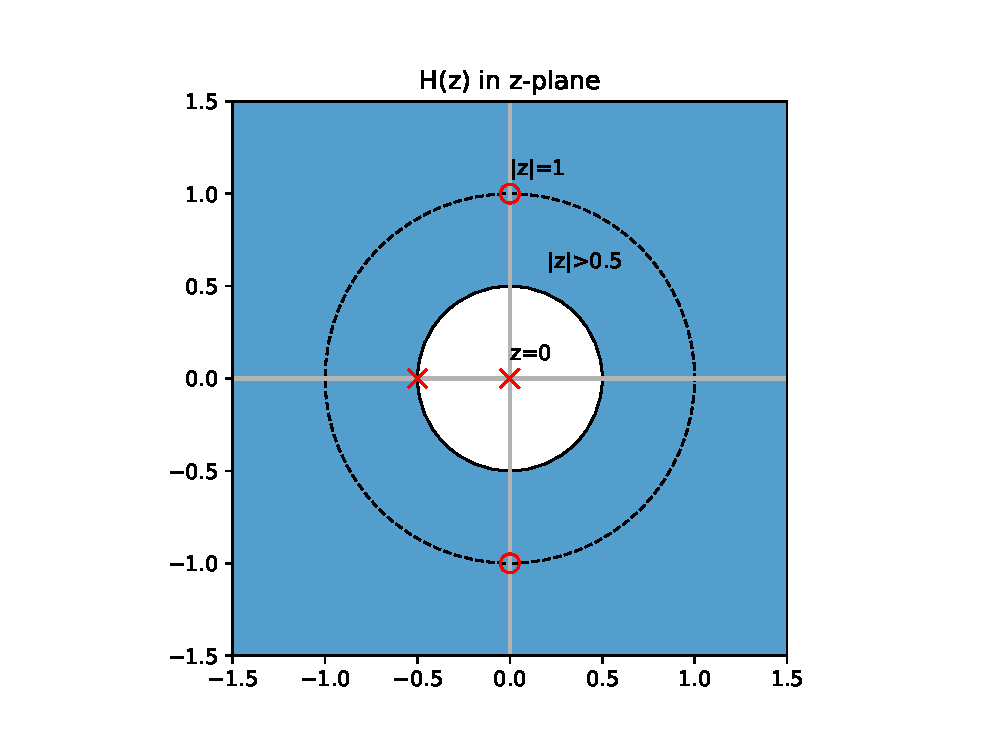
\includegraphics[width=11cm]{./figs/z_plane.eps}
    \caption{H(z) in z-plane}
    \label{Z_plane analysis}
\end{figure}
From the figure.\ref{Z_plane analysis}, we can observe that ROC includes the unit circle $\abs{z} = 1$, which implies the given IIR filter is stable, because h(n) is absolutely summable.\\
Verification:- Given bounded input x(n).,
\begin{align}
    x(n) = \cbrak{\underset{\uparrow}{1},2,3,4,2,1}\\
    y(n)+\frac{1}{2}y(n-1) = x(n)+x(n-2)
\end{align}
\begin{figure}[h!]
    \centering
    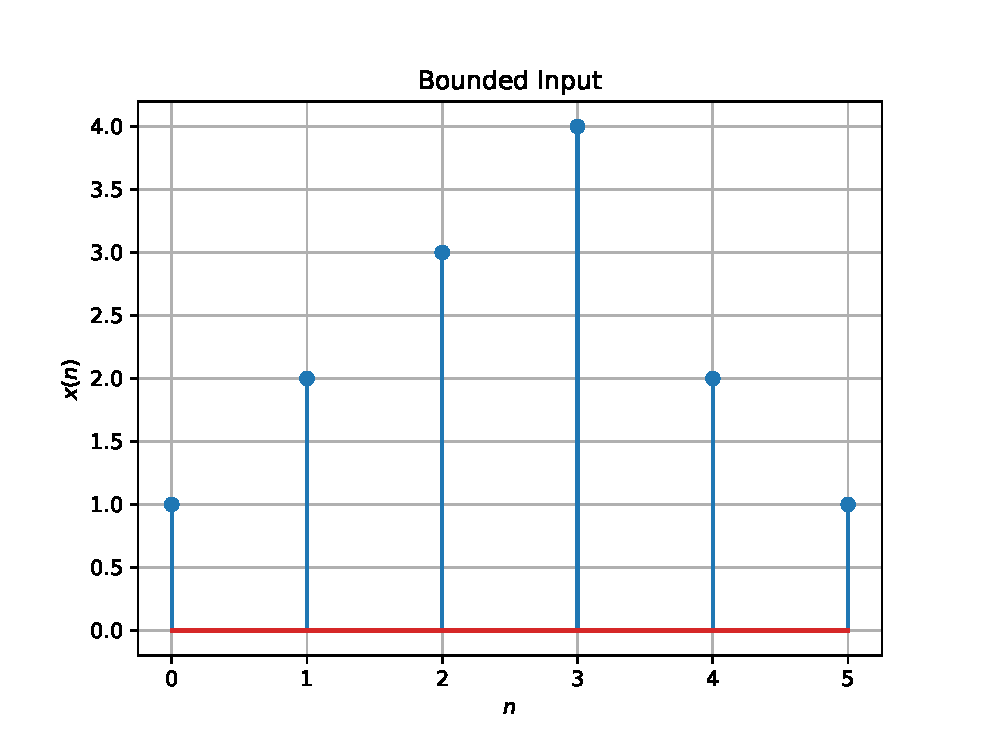
\includegraphics[width=8cm]{./figs/x_n.eps}
    \caption{Given bounded input}
    \label{xn}
\end{figure}
Maximum value of x(n) is 4 and minimum value of x(n) is
0. x(n) is bounded.\\
From the python code,the maximum value of y is 4.375. Minimum value of y is -0.449. y(n) vanishes to zero as n tends to infinity. Therefore, output is bounded.\\
\begin{figure}[h!]
    \centering
    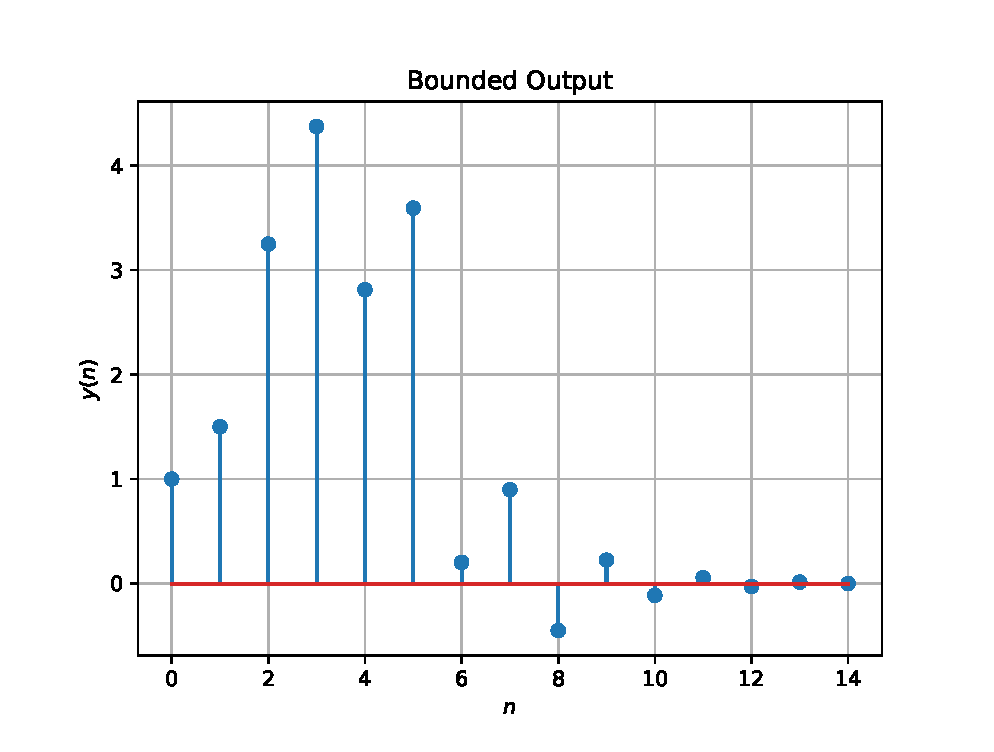
\includegraphics[width=8.5cm]{./figs/y_n.eps}
    \caption{Bounded output}
    \label{yn}
\end{figure}
The system returns bounded output for the given bounded input. Implies, the system is stable.\\ Hence, verified.
\end{document}
